\documentclass[11pt]{article}
\usepackage{amsmath, amssymb, amsthm}
\usepackage[retainorgcmds]{IEEEtrantools}

\usepackage[pdftex]{graphicx}
\usepackage{tikz}
\usetikzlibrary{intersections,decorations.pathmorphing}

\usepackage{fancyhdr}

%Format stuff
\pagestyle{fancy}
\headheight 35pt

%Header info
\chead{\Large \textbf{Dampened Oscillators}}
\lhead{}
\rhead{}

\begin{document}
\begin{center}
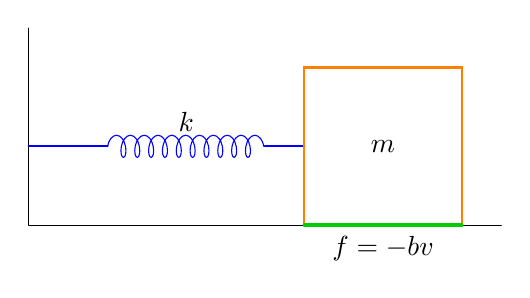
\begin{tikzpicture}
	[scale=1,line cap=round,
	%Styles
	axes/.style=,
	important line/.style={very thick},
	information text/.style={rounded corners,fill=red!10,inner sep=1ex},
	dot/.style={circle,inner sep=1pt,fill,label={#1},name=#1},
	spring/.style={decorate, draw=blue,decoration={coil,amplitude=4pt, segment length=5pt}}			
	]
	
	%Colors
	\colorlet{anglecolor}{green!50!black}	%angle arcs/lines
	
	%The graphic
	\draw[black] (0,0) -- (0, 2.5);
	\draw[black] (0, 0) -- (6, 0);	
	
	\draw[blue,thick] (0, 1) -- (1, 1);
	\draw[spring] (1, 1) -- node[above=2pt,black] {$k$} (3, 1);
	\draw[blue,thick] (3, 1) -- (3.5, 1);
	
	\draw[orange,thick] (3.5, 0) rectangle (5.5, 2);
	\node (m) at (4.5, 1) {$m$};
	
	\draw[green!80!black,very thick] (3.5, 0) -- node[below,black] {$f = -bv$}(5.5, 0);
\end{tikzpicture}
\end{center}
\section{Equation of Motion}
	\begin{IEEEeqnarray}{rCl}
		\ddot{x} + \gamma\dot{x} + \omega_0^2 x & = & 0\\
		\gamma & = & \frac{b}{m}\\
		\omega_0^2 & = & \frac{k}{m}
	\end{IEEEeqnarray}
	
	Solving for the above differential equation (by assuming $x$ is an oscillating function itself in the form $Ae^i{\omega t + \delta}$ and doing the algebra), we get the following solution.
	\begin{equation}
		x(t) = Ae^{-\omega_i t}e^{i(\omega_r t + \delta)}
	\end{equation}
	\begin{equation}
		\omega_i = \frac{\gamma}{2}
	\end{equation}
	\begin{equation}
		\omega_r^2 = \omega_0^2 - \frac{\gamma^2}{4}
	\end{equation}
	
	Note that $\omega$ for the oscillating frequency of the system is a complex number, defined as $\omega = \omega_r + i\omega_i$. 
	
	Graphically, the equation of motion for a dampened oscillator is a periodic wave that decreases in magnitude along two horizontal asymptotes, the graphs of $\pm Ae^{-\omega_i t}$.
	
\section{Energy}
	For a lightly dampened system, because $\omega \approx \omega_0$ for short periods of time, we can calculate the energy of the system pretty simply.
	\begin{IEEEeqnarray}{rCl}
		E(t) & = & E_0 e^{-\gamma t}\\
		E_0 & = & \frac{1}{2}m\omega_0^2A^2
	\end{IEEEeqnarray}
	
\section{Q Factor}
	The Q factor, or quality factor, of a dampened oscillator measures the quality of the system. A higher Q factor means that the system will store energy for longer while a lower Q factor means that the system quickly loses energy to heat. The Q factor is the inverse of the fraction of energy lost when the phase advances 1 radian.
	\begin{equation}
		t_1 = \frac{1}{\omega_0}
	\end{equation}
	
	Letting $t_1$ be the amount of time that it takes for the system to advance 1 radian, we know that the ratio of energy at a given time $t$ to the original energy is, for lightly dampened systems,
	\begin{equation}
		\frac{E(t)}{E_0} \approx e^{-\gamma t} \approx 1 - \gamma t
	\end{equation}
	
	Therefore, the fraction of energy lost is $\gamma t$, and 
	\begin{equation}
		Q = \frac{\omega_0}{\gamma}
	\end{equation}
%	\begin{center}
%	\begin{tikzpicture}
%		[scale=3,line cap=round,
%		%Styles
%		axes/.style=,
%		important line/.style={very thick},
%		information text/.style={rounded corners,fill=red!10,inner sep=1ex},
%		dot/.style={circle,inner sep=1pt,fill,label={#1},name=#1}			
%		]
%		
%		%Colors
%		\colorlet{anglecolor}{green!50!black}	%angle arcs/lines
%		
%		%The graphic
%	\end{tikzpicture}
%	\end{center}

%	\begin{figure}[htb]
%		\centering
%		\includegraphics[width=0.8\textwidth]{filename.eps}
%		\caption{Caption.}
%		\label{fig:figure}
%	\end{figure}

%		\def\enotesize{\normalsize}
%		\theendnotes
\end{document}